\begin{multicols}{3}
\byline{``Chained Rose''}{Зорница, 12 Б}
Здравейте! Аз съм Зорница Михалева и ще ви споделя една история за осъществени 
мечти. За времето, в което бяхме заедно с Мартин Стефанов (китара), Иван Василев 
(ритъм китара), Вълчо Иванов (бас), и Никола Фучеджиев (барабани) в една рок 
група, ние изживяхме едно четиригодишно приключение. 
Нашето име е  “Chained Rose”, което в превод означава „окована роза“. Идеята за 
стартиране на такава банда беше на момчетата, с тях се запознах, когато бях 
първа година в гимназията. Моята история се преплете с техните, когато се 
намерих без учебници за началото на учебната година. Запознах се с едно от 
момчетата, което ме снабди със старите си учебници, и по-късно след като разбра, 
че пея в хор, ме представи на своите приятели, които искаха да направят група. 
Не след дълго започнахме репетиции в едно студио-мазе извън училище. Самата идея 
аз да музицирам със съученици беше по-вълнуваща от всичко. И петимата бяхме 
пленени от връзката, която успяхме бързо да осъществим един с друг, и неусетно 
създадохме красиво и стабилно приятелство. Първото ни участие беше на Kоледно 
тържество в училище на втория етаж, където публиката беше много въодушевена, че 
вече в гимназията ни има рок група. Интересът към нас се усилваше с по-честите 
концерти на гимназията, в които участвахме. След време, в което репетициите 
ставаха по-дълги и репертоарът ни растеше, ние решхме да организираме в бургаски 
клуб свой собствен концерт. Енергията ни заразяваше публиката и все повече хора 
от всички възрасти посещаваха наши участия. Изведнъж беше станала голяма мода да 
се събират деца в групи и да свирят свои любими песни. За три дълги години 
публиката се радваше на насъбралите се тийн групи, които с радост организираха 
всеки уикенд концерти в бургаските зали и клубове. През това време от Chained 
Rose започнахме да представяме и наши песни, които бързо биваха запаметявани от 
фенове и скоро хората пееха с нас. Когато това се случваше, изпитвах такава 
гордост и радост към моите приятели, с които правехме това, което обичаме и без 
страх го споделяме с хората срещу нас. Не веднъж съм плакала от радост зад 
колисите. Не веднъж сме чувствали силна умора след концерт, но всички тези 
споделени положителни емоции с публиката и между всеки един от нас ни водеха 
напред и ни давха сили да продължим. Участвали сме в конкурси като “Поп/Рок 
Несебър” и “Battle of the Bands” в Бургас и „Голямо Междучасие 4“ в София, 
където сме награждавани най-вече с гласовете на публиката и с невероятните 
купони, където групата и публиката се сливахме в емоцията от изкуството, което 
всички толкова обичаме. През 2012 година на фестивала “July Morning” излязохме 
на сцена на плажа наред с известни български музиканти и в рамките на половин 
час се радвахме на овации както от наши фенове, така и от хора, пътували 
специално за фестивала. В началото на 2013 година записахме в студио три от 
нашите авторски песни, които са известни все още сред публиката. Трима от екипа 
ни завършиха гимназията през 2014г., което бележи края на едно прекрасно 
пътешествие. Иван и Вълчо продължават образованието си в столицата ни, а Никола 
замина за Дания. Мартин и аз сме абитуриенти тази година, в която училището ни 
празнува 55-тия си рожден ден. 
Не бих могла да опиша с думи колко много ми донесе участието в група като тази, 
която успяхме да съхраним толкова време. С взаимна подкрепа и обич се потапяхме 
в дълбините на музиката и сбъдвахме своите мечти всеки един път когато излизахме 
на сцена пред публика или репетирахме с часове заедно. Тези емоции ще си 
спомняме след години. Тези приятелства ще ни останат вечни, защото колкото 
повече любов дарявахме с музиката си, толкова обич споделяхме и на сцената. Обич 
към музиката, обич към публиката, обич между всеки един от нас. 
Можете да намерите наша музика, снимки и видеа на официалните ни страници: 
facebook.com/chainedroseband, 
\small{youtube.com/user/chainedroseband}
\end{multicols}

\begin{center}
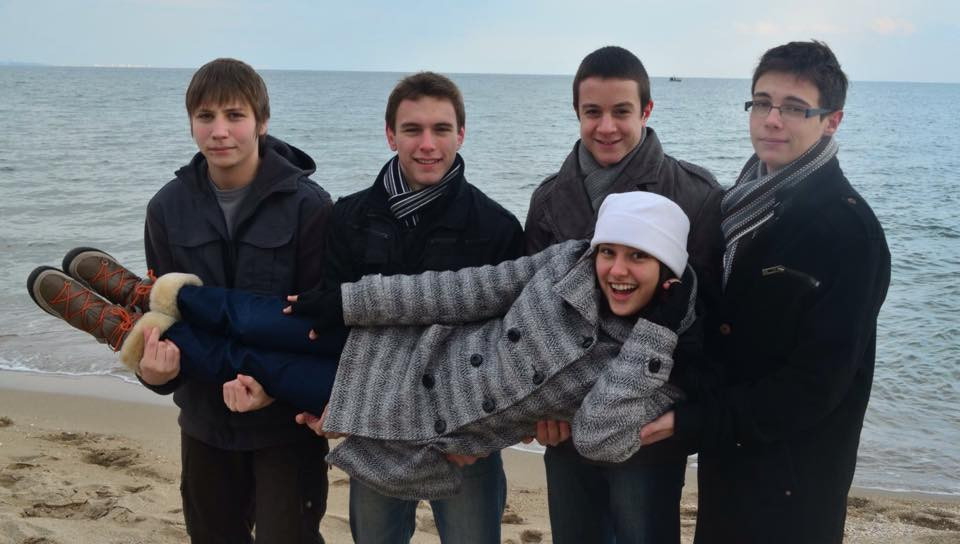
\includegraphics[width=5.7in]{./Chained_Rose/CR.jpg}
\end{center}

\closearticle
